\documentclass[11pt]{article}
\usepackage{amsmath, amssymb, amsthm}
\usepackage[retainorgcmds]{IEEEtrantools}

\usepackage[pdftex]{graphicx}
\usepackage{tikz}
\usetikzlibrary{intersections, calc}

\usepackage{fancyhdr}

%Format stuff
\pagestyle{fancy}
\headheight 35pt

%Header info
\chead{\Large \textbf{Simple Harmonic Oscillators}}
\lhead{}
\rhead{}

\begin{document}
\section{Mass-Spring (Horizontal)}
	\subsection{Motion}
		Consider a simple harmonic oscillator (SHO) like a horizontal mass-spring system. Force is given by Hooke's Law, $F=-kx$ where $x$ is the displacement from equilibrium.
		\begin{IEEEeqnarray}{rCl}
			F & = & -kx\\
			ma & = & -kx\\
			m\ddot{x} & = & -kx
		\end{IEEEeqnarray}
		The general equations of motion for a SHO, after solving for the second-order differential equation above, are as follows.
		\begin{IEEEeqnarray}{rCl}
			0  & = & \ddot{x} + \frac{k}{m}x\\
			x(t) & = & A\cos(\omega t + \delta)
		\end{IEEEeqnarray}
		Where $A$ is amplitude, in meters, given by the initial position, $\omega$ is angular frequence, in Hz, and $\delta$ is phase, given by the initial velocity, in radians. Plugging the general solution into the differential equation, we can determine that
		\begin{equation}
			\omega = \sqrt{\frac{k}{m}}
		\end{equation}
		
	\subsection{Energy}
		Straightforward equations for potential and kinetic energy by displacement:
		\begin{IEEEeqnarray}{rCl}
			U(x) & = & \frac{1}{2} kx^2\\
			KE(x) & = & \frac{1}{2}m\dot{x}^2
		\end{IEEEeqnarray}
		
		Substituting for $x$ to express these equations by time:
		\begin{IEEEeqnarray}{rCl}
			U(t) & = & \frac{1}{2}k[A\cos(\omega t + \delta)]^2\\
			KE(t) & = & \frac{1}{2}m[-A\omega \sin(\omega t + \delta)]^2
		\end{IEEEeqnarray}
		
		After adding the above two equations together, the total energy of the system is then
		\begin{equation}
			\sum E = \frac{1}{2} kA^2
		\end{equation}
		
\section{Harmonic Potentials}
	Quadratic potential functions $U(x)$ give rise to simple harmonic motion. Considering the case of an arbitrary $U(x)$, expanding a Taylor series at points of stable equilibrium (local minima) $U(x_0)$ shows that the potential can be approximated by a quadratic function for small displacements.
	\begin{IEEEeqnarray}{rCl}
		U(x_0) \approx U(x_o + a) =  U(a) & = & U(x_0) + U'(x_0)a + \frac{1}{2}U''(x_0)a^2 + \ldots\\
		& \approx & U(x_0) + \frac{1}{2}U''(x_0)a^2
	\end{IEEEeqnarray}
	
	Thus, for an arbitrary $U(x)$, the natural frequency of small oscillations can be approximated by 
	\begin{equation}
		\omega \approx \sqrt{\frac{U''(x_0)}{m}}
	\end{equation}
	
\section{Plane Pendulum}
	\begin{center}
	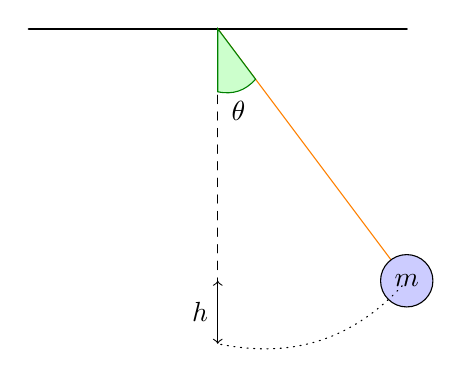
\begin{tikzpicture}
		[scale=.8,line cap=round,
		%Styles
		axes/.style=,
		important line/.style={very thick},
		information text/.style={rounded corners,fill=red!10,inner sep=1ex},
		dot/.style={circle,inner sep=1pt,fill,label={#1},name=#1},
		mass node/.style={circle,fill=blue!20,draw}		
		]
		
		%Colors
		\colorlet{anglecolor}{green!50!black}	%angle arcs/lines
		
		%The graphic
		
		\coordinate (origin) at (0, 0);
		\coordinate (mass) at (3, -4);
		\coordinate (ground) at (0, -5);
		
		\draw[thick] (-3, 0) -- (3, 0);
		\draw[dashed] (origin) -- (ground);
		\draw[orange] (origin) -- (mass);
		
		\node[mass node] (M) at (mass) {$m$};
		\draw[dotted] (mass) to [bend left] (ground);
		
		\filldraw[fill=green!20, draw=anglecolor] (origin) -- ($(origin)!1cm!(ground)$) to [bend right] node[below, black] {$\theta$} ($(origin)!1cm!(mass)$) -- cycle;
		
		\draw[<->,black] (ground) -- node[left] {$h$} (0, -4);
		
	\end{tikzpicture}
	\end{center}
	
	\subsection{Motion}	
		\begin{IEEEeqnarray}{rCl}
			\tau & = & -F\times l = -mgl\sin\theta\\
			\tau & = & I\ddot{\theta}
		\end{IEEEeqnarray}
		
		When $\theta$ is small, $\sin\theta \approx \theta$. Knowing this, the plane pendulum becomes another example of a SHO.
		\begin{IEEEeqnarray}{rCl}
			0 & = & \ddot{\theta} + \frac{g}{l}\sin\theta\\
			\sin\theta & \approx & \theta\\
			\omega_0 & \approx & \sqrt{\frac{g}{l}}
		\end{IEEEeqnarray}
		
	\subsection{Energy}
		\begin{IEEEeqnarray}{rCl}
			U(h) & = & mgh\\
			h & = & l - l\cos\theta\\\nonumber\\
			U(\theta) & = & mgl(1 - \cos\theta)\\
			U''(\theta) & = & mgl\cos\theta
		\end{IEEEeqnarray}
		
		At $x_0 = 0$, $U'' = mgl$. Because the system is rotational, instead of using the mass as the denominator in the radical for the frequency of oscillation, use $I$, the rotational analog of mass.
		\begin{equation}
			\omega_0 = \sqrt{\frac{mgl}{I}}
		\end{equation}
		\begin{equation}
			I = ml^2
		\end{equation}

%	\begin{figure}[htb]
%		\centering
%		\includegraphics[width=0.8\textwidth]{filename.eps}
%		\caption{Caption.}
%		\label{fig:figure}
%	\end{figure}

%		\def\enotesize{\normalsize}
%		\theendnotes
\end{document}